% TeX template for writing thesis
% Islamic Azad University
% Auhtor of this template: Mir, A.
% Nov 30, 2018
% https://github.com/mir-am/IAU-Thesis-TeX-Template

\documentclass[10pt,a4paper]{report}

% Packages
% Uncomment a package if you want to use it.
\usepackage[top=35mm, bottom=30mm, left=25mm, right=35mm]{geometry} % Page margins
\usepackage{graphicx} % For inserting images into document
\usepackage[final]{pdfpages} % For inserting PDF file
\usepackage{amsfonts, amsmath, amssymb, amsthm} % Math symbols
%\usepackage[nodisplayskipstretch]{setspace} % For vertical space between equations
\usepackage[xindy, acronym, nonumberlist=true]{glossaries}
\usepackage{subfig} % For side-by-side figures
\usepackage{booktabs} % For tables
\usepackage{threeparttable}
\usepackage{rotating}
\usepackage{footnote} % To insert a footnote in the table enviroment
\usepackage{enumitem}
\usepackage[font={small}]{caption}
\usepackage{fancyhdr} % To insert sections titles in pages' headers
\usepackage[subfigure, titles]{tocloft} % To customize Table of contents
\usepackage[hidelinks]{hyperref} % To generate hyperlinks for sections, figures, etc.
\usepackage[ruled, algochapter]{algorithm2e} % To write algorithms and pseudo-code
%\usepackage{etoolbox}

% XePersian for writing Persian content
% This package should be loaded after above packages.
\usepackage{xepersian} 

%%%%%%%%%%%%%%%%%%%%%%%

% Xepersian settings
\settextfont[Scale=1.4]{B Lotus}
\setlatintextfont[Scale=1]{Times New Roman}
\setdigitfont[Scale=1.2]{XB Niloofar}

% Definitions
% Custom definitions
% DO NOT CHANGE THESE SETTINGS UNLESS YOU KNOW WHAT YOU ARE DOING.

\makeatletter
\bidi@patchcmd{\@Abjad}{آ}{الف}
{\typeout{Succeeded in changing `آ` into `الف`}}
{\typeout{Failed in changing `آ` into `الف`}}
\makeatother
\PersianAlphs

% Table of content modification
\setcounter{secnumdepth}{3}
\setcounter{tocdepth}{3} % To show subsubsections in TOC
\newcommand\notation[2]{#1\dotfill\lr{#2}\\}
\renewcommand{\cftchapleader}{\cftdotfill{\cftdotsep}}
% Solves overlapping numbers and sec titles
\setlength{\cftsubsecnumwidth}{2.5em}
\setlength{\cftsubsubsecnumwidth}{3.5em}
\SepMark{-}

% Names of lists
\renewcommand{\bibname}{مراجع}
\renewcommand{\listfigurename}{فهرست شکل‌ها}

%%%%%%%%%%%%%%%%%%%%%%%%%%%%%

% Folder that contains Figures
\graphicspath{{figs/}}

%\everymath\expandafter{\the\everymath\PersianMathsDigits\SetMathsDigits}
%\DefaultMathsDigits

% Table settings
% Space between rows of tables
\renewcommand{\arraystretch}{1.5}
\newcommand{\ra}[1]{\renewcommand{\arraystretch}{#1}}

% Define size of columns of table
\newcommand{\acol}{p{2.10cm}}
\newcommand{\tcol}{p{1.20cm}}

%%%%%%%%%%%%%%%%%%%%%%%%%%%%%

% Algorithms and its TOC
\renewcommand{\algorithmcfname}{الگوریتم}
\renewcommand{\listalgorithmcfname}{فهرست الگوریتم‌ها}

% For writing steps in the algorithm enviroment.
\newenvironment{steps}
{
\begin{minipage}{.92\linewidth}
\baselineskip=0.9cm
}{
\end{minipage}
}

%%%%%%%%%%%%%%%%%%%%%%%%%%%%%

% Glossaries settings
% Styles
% Persian to English style
\newglossarystyle{myFaToEn}{%
	\renewenvironment{theglossary}{}{}
	\renewcommand*{\glsgroupskip}{\vskip 10mm}
	\renewcommand*{\glsgroupheading}[1]{\subsection*{\glsgetgrouptitle{##1}}}
	\renewcommand*{\glossentry}[2]{\noindent\glsentryname{##1}\dotfill\space \glsentrytext{##1}
		
	}
}

% English to Persian style
\newglossarystyle{myEntoFa}{%
	\renewenvironment{theglossary}{}{}
	\renewcommand*{\glsgroupskip}{\vskip 10mm}
	\renewcommand*{\glsgroupheading}[1]{\begin{latin} \subsection*{\glsgetgrouptitle{##1}} \end{latin}}

	\renewcommand*{\glossentry}[2]{\noindent\glsentrytext{##1}\dotfill\space \glsentryname{##1} \\
	}
}

% Abbreviations style
\newglossarystyle{myAbbrlist}{%
	
	\renewenvironment{theglossary}{}{}
	\renewcommand*{\glsgroupskip}{\vskip 10mm}
	\renewcommand*{\glsgroupheading}[1]{\begin{latin} \subsection*{\glsgetgrouptitle{##1}} \end{latin}}

	\renewcommand*{\glossentry}[2]{\begin{latin} \noindent\glsentrytext{##1}\dotfill\space \Glsentrylong{##1} \end{latin}}

	\renewcommand*{\acronymname}{\rl{فهرست اختصارات}}
}

% Files
\newglossary[glg]{english}{gls}{glo}{واژه‌نامه انگلیسی به فارسی}
\newglossary[blg]{persian}{bls}{blo}{واژه‌نامه فارسی به انگلیسی}
\makeglossaries
\glsdisablehyper

% Redefintion of commands
\let\oldgls\gls
\let\oldglspl\glspl

\makeatletter

\renewrobustcmd*{\gls}{\@ifstar\@msgls\@mgls}
\newcommand*{\@mgls}[1] {\ifthenelse{\equal{\glsentrytype{#1}}{english}}{\oldgls{#1}\glsuseri{f-#1}}{\lr{\oldgls{#1}}}}
\newcommand*{\@msgls}[1]{\ifthenelse{\equal{\glsentrytype{#1}}{english}}{\glstext{#1}\glsuseri{f-#1}}{\lr{\glsentryname{#1}}}}

\renewrobustcmd*{\glspl}{\@ifstar\@msglspl\@mglspl}
\newcommand*{\@mglspl}[1] {\ifthenelse{\equal{\glsentrytype{#1}}{english}}{\oldglspl{#1}\glsuseri{f-#1}}{\oldglspl{#1}}}
\newcommand*{\@msglspl}[1]{\ifthenelse{\equal{\glsentrytype{#1}}{english}}{\glsplural{#1}\glsuseri{f-#1}}{\glsentryplural{#1}}}

\makeatother

\newcommand{\newword}[4]{
	\newglossaryentry{#1}     {type={english},name={\lr{#2}},plural={#4},text={#3},description={}}
	\newglossaryentry{f-#1} {type={persian},name={#3},text={\lr{#2}},description={}}
}

% Footnote for first occurence of a word
\defglsentryfmt[english]{\glsgenentryfmt\ifglsused{\glslabel}{}{\LTRfootnote{\glsentryname{\glslabel}}}}
\defglsentryfmt[acronym]{\glsentryname{\glslabel}\ifglsused{\glslabel}{}{\LTRfootnote{\glsentrydesc{\glslabel}}}}

% Print glossaries and abbrevations
\newcommand{\printabbreviation}{
	\cleardoublepage
	\phantomsection
	\baselineskip=.75cm
	
	\addcontentsline{toc}{chapter}{فهرست اختصارات}
	\setglossarystyle{myAbbrlist}
	\begin{LTR}
		\Oldprintglossary[type=acronym]	
	\end{LTR}
	\clearpage
}%

\newcommand{\printacronyms}{\printabbreviation}

\let\Oldprintglossary\printglossary
\renewcommand{\printglossary}{
	\let\appendix\relax

	\clearpage
	\phantomsection
	\baselineskip=.75cm
	
	\twocolumn{}
	
	\addcontentsline{toc}{chapter}{واژه نامه انگلیسی به فارسی}
	\setglossarystyle{myEntoFa}
	\Oldprintglossary[type=english]
	
	\clearpage
	\phantomsection

	\addcontentsline{toc}{chapter}{واژه نامه فارسی به انگلیسی}
	\setglossarystyle{myFaToEn}
	\Oldprintglossary[type=persian]
	\onecolumn{}
}%


% end of glossaries settings
%%%%%%%%%%%%%%%%%%%%%%%%%%%%%

%\title{}
%\author{}

% glossaries
% My glossaries and abbreviations

% Glossaries
\newword{ML}{Machine learning}{یادگیری ماشین}{}
\newword{AI}{Artificial intelligence}{هوش مصنوعی}{}


% Abbreviations
\newacronym{SVM}{SVM}{Support Vector Machine}
\newacronym{QPP}{QPP}{Quadratic Programming Problem}



\begin{document}
\baselineskip=0.9cm % Space between lines
%\maketitle

%Front page
\thispagestyle{empty}

% Azad University logo
\centerline{
\includegraphics[height=5cm]{figs/logo.png}}

\begin{center}
\vspace{0.5cm}

\textbf{دانشگاه آزاد اسلامی}
\\[.2cm]
\textbf{واحد تهران شمال}
\\[0.5cm]

دانشکده برق و مهندسی کامپیوتر گروه مهندسی کامپیوتر
\\[.5cm]
پایان‌نامه برای دریافت درجه کارشناسی ارشد «\lr{M.Sc}»
\\[.2cm]
رشته مهندسی کامپیوتر، گرایش ...............
\\[0.5cm]

{\Large
\textbf{عنوان}
}
\\
قالب \lr{TeX} برای نوشتن پایان‌نامه
\\[0.5cm]

{\Large
	\textbf{استاد راهنما}
}
\\
...............
\vskip 0.5cm

{\Large
	\textbf{استادان مشاور}
}
\\
...............
\vskip 0.5cm
{\Large
	\textbf{نگارش}
}
\\
...............
\vskip 0.5cm
پاییز ۱۳۹۷
\end{center}

% Besm page
% Besm page

\thispagestyle{empty}

\begin{center}
\vskip 8cm


\includegraphics{figs/besm}

\end{center}

\newpage

% Statement of originalty
% Statement of orginalty
\thispagestyle{empty}
\noindent

\textbf{\Large تعهدنامه اصالت  پایان‌نامه}
\vskip 1cm

\noindent اینجانب ........................ دانش آموخته مقطع کارشناسی ارشد ناپیوسته/دکترای تخصصی در رشته مهندسی کامپیوتر که در تاریخ ........................ از پایان نامه/ رساله خود تحت عنوان " .............." با کسب نمره ............ و درجه ................... دفاع نموده‌ام بدین‌وسیله متعهد می‌شوم:
\begin{enumerate}
	\item این پایان نامه/ رساله حاصل تحقیق و پژوهش انجام شده توسط اینجانب بوده و در مواردی که از دستاوردهای علمی و پژوهشی دیگران (اعم از پایان نامه، کتاب،مقاله و....) استفاده نموده‌ام، مطابق ضوابط و رویه موجود، نام منبع مورد استفاده و سایر مشخصات آن را در فهرست مربوطه ذکر و درج کرده‌ام.
	\item این پایان نامه/ رساله قبلا برای دریافت هیچ مدرک تحصیلی (هم سطح،پایین تر یا بالاتر) در سایر دانشگاه‌ها و موسسات آموزشی عالی ارائه نشده است.
	\item 	چنانچه بعد از فراغت تحصیل، قصد استفاده و هرگونه بهره برداری اعم از چاپ کتاب،ثبت اختراع و... از این پایان نامه داشته باشم،از حوزه معاونت پژوهشی واحد مجوزهای مربوطه را اخذ نمایم.
	\item 	چنانچه در هر مقطعی زمانی خلاف موارد فوق ثابت شود، عواقب ناشی از آن را می‌پذیرم و واحد دانشگاهی مجاز است با اینجانب مطابق ضوابط و مقررات رفتار نموده و در صورت ابطال مدرک تحصیلی‌ام هیچگونه ادعایی نخواهم داشت.
\end{enumerate}

\vskip 0.5cm
\begin{flushleft}
\textbf{نام و نام خانوادگی: .................}
\end{flushleft}

% Research Morality
% 
\thispagestyle{empty}

\includepdf[pages=-]{misc/Manshor.pdf}

\thispagestyle{empty}

\noindent
\textbf{\Large تقدیم به:}
\vskip 1cm

\newpage
\thispagestyle{empty}

\begin{center}
\textbf{\Large سپاسگزاری}
\end{center}
\vskip 1cm
\noindent در اینجا می‌توانید از اشخاص و سازمان‌ها تشکر کنید.

\vskip 1cm


\pagenumbering{alph}

% Lists
\tableofcontents
\listoftables
\listoffigures
% If you have alogrithms in your thesis, uncomment following command.
%\listofalgorithms

% Lists customization
\addtocontents{toc}{\textbf{عنوان}~\hfill\textbf{صفحه}\par}
\addtocontents{lot}{\textbf{عنوان}~\hfill\textbf{صفحه}\par}
\addtocontents{lof}{\textbf{عنوان}~\hfill\textbf{صفحه}\par}
%\addtocontents{loa}{\textbf{عنوان}~\hfill\textbf{صفحه}\par} % For list of algorithms.

% Notations
% Uncomment this if you want to display list of notations 
%% List of Notations. This is an optional list.

\chapter*{فهرست علائم و نمادها}\markboth{فهرست علائم و نمادها}{فهرست علائم و نمادها}

\baselineskip=0.8cm

\notation{مجموعه داده آموزشی}{$T$}
\notation{نماد مجانبی}{$\mathcal{O}(\ .\ )$}

% Reset line space for main content
\baselineskip=0.9cm

% Persian Abstarct

\thispagestyle{plain}
\pagenumbering{arabic}

% Adding abstract to TOC
\phantomsection
\addcontentsline{toc}{chapter}{چکیده}

\section*{چکیده}
چکیده پایان نامه را در اینجا بنویسید.

%همچنین با بکارگیری روش کمترین مربعات، مدل خروجی در دسته‌بند \lr{KNN-LSTSVM} با حل کردن دو دستگاه معادلات خطی بدست می‌آید. بطوریکه سرعت یادگیری این دسته‌بند به طور قابل توجه‌ای افزایش یافته است. دسته‌بند \lr{RKNN-TSVM} به نمونه‌ها براساس فاصله بین نزدیک‌ترین همسایه‌هایشان وزن می‌دهد و ریسک ساختاری را در مسئله بهینه‌سازی کمینه می‌کند.

\vskip 2cm
\noindent
\textbf{واژه‌های کلیدی:} 
قالب \lr{TeX}، هوش مصنوعی


% Chapters
% This adds a rule bar and sections title to header.
\pagestyle{fancy}
\fancyhf{}
\cfoot{\thepage}
\fancyhead[R]{\rightmark}

\chapter{کلیات} \label{ch:1}
\section{مقدمه} \label{sec:1:1}
\gls{ML} یکی از شاخه‌های پرکاربرد \gls{AI} است \cite{jordan2015}.

\section{تعریف مسئله} \label{sec:1:2}


\section{نوآوری‌های پژوهش} \label{sec:1:3}
نوآوری‌های این پژوهش عبارتند از:
\begin{enumerate}
	\item مورد اول
	
	\item مورد دوم
\end{enumerate}

\section{ساختار کلی  پایان‌نامه}\label{sec:1:4}
در فصل \ref{ch:2}، کارهای پیشین مرور شده است.

روش پیشنهادی در فصل \ref{ch:3} ارائه شده است. 

در فصل \ref{ch:4}، روش پیشنهادی ارزیابی و بررسی شده است.


در فصل آخر، یافته‌های اصلی پژوهش مرور شده است.
\newpage


% Chapter 2 Support Vector Machine

\chapter{پشینیه پژوهش} \label{ch:2}

\section{ماشین بردار پشتیبان} \label{sec:2:1}

ماشین بردار پشتیبان (\gls{SVM}) با هدف جداسازی نمونه‌های دو کلاس توسط کورتس\LTRfootnote{Cortes} و وپنیک\LTRfootnote{Vapnik} در سال 1995 معرفی گردید \cite{vapnik1995}. این دسته‌بند برای بدست آوردن ابرصفحه بهینه، یک مسئله برنامه‌ریزی درجه دو (\gls{QPP}) حل می‌کند که در رابطه \ref{eq:2:1} ذکر شده است.

\begin{equation}
\begin{gathered} 
\mathop{min}\limits_{w}\frac{1}{2}{{\left\| w \right\|}^{2}} \\
\textrm{\lr{s.t. }} {{y}_{i}}({{w}^T}{{x}_{i}}+b)\ge 1,\forall i
\end{gathered}
\label{eq:2:1}
\end{equation}

شکل \ref{fig:SVM} تفسیر هندسی دسته‌بند را نشان می‌دهد.

\begin{figure}[!h]
	\centering
	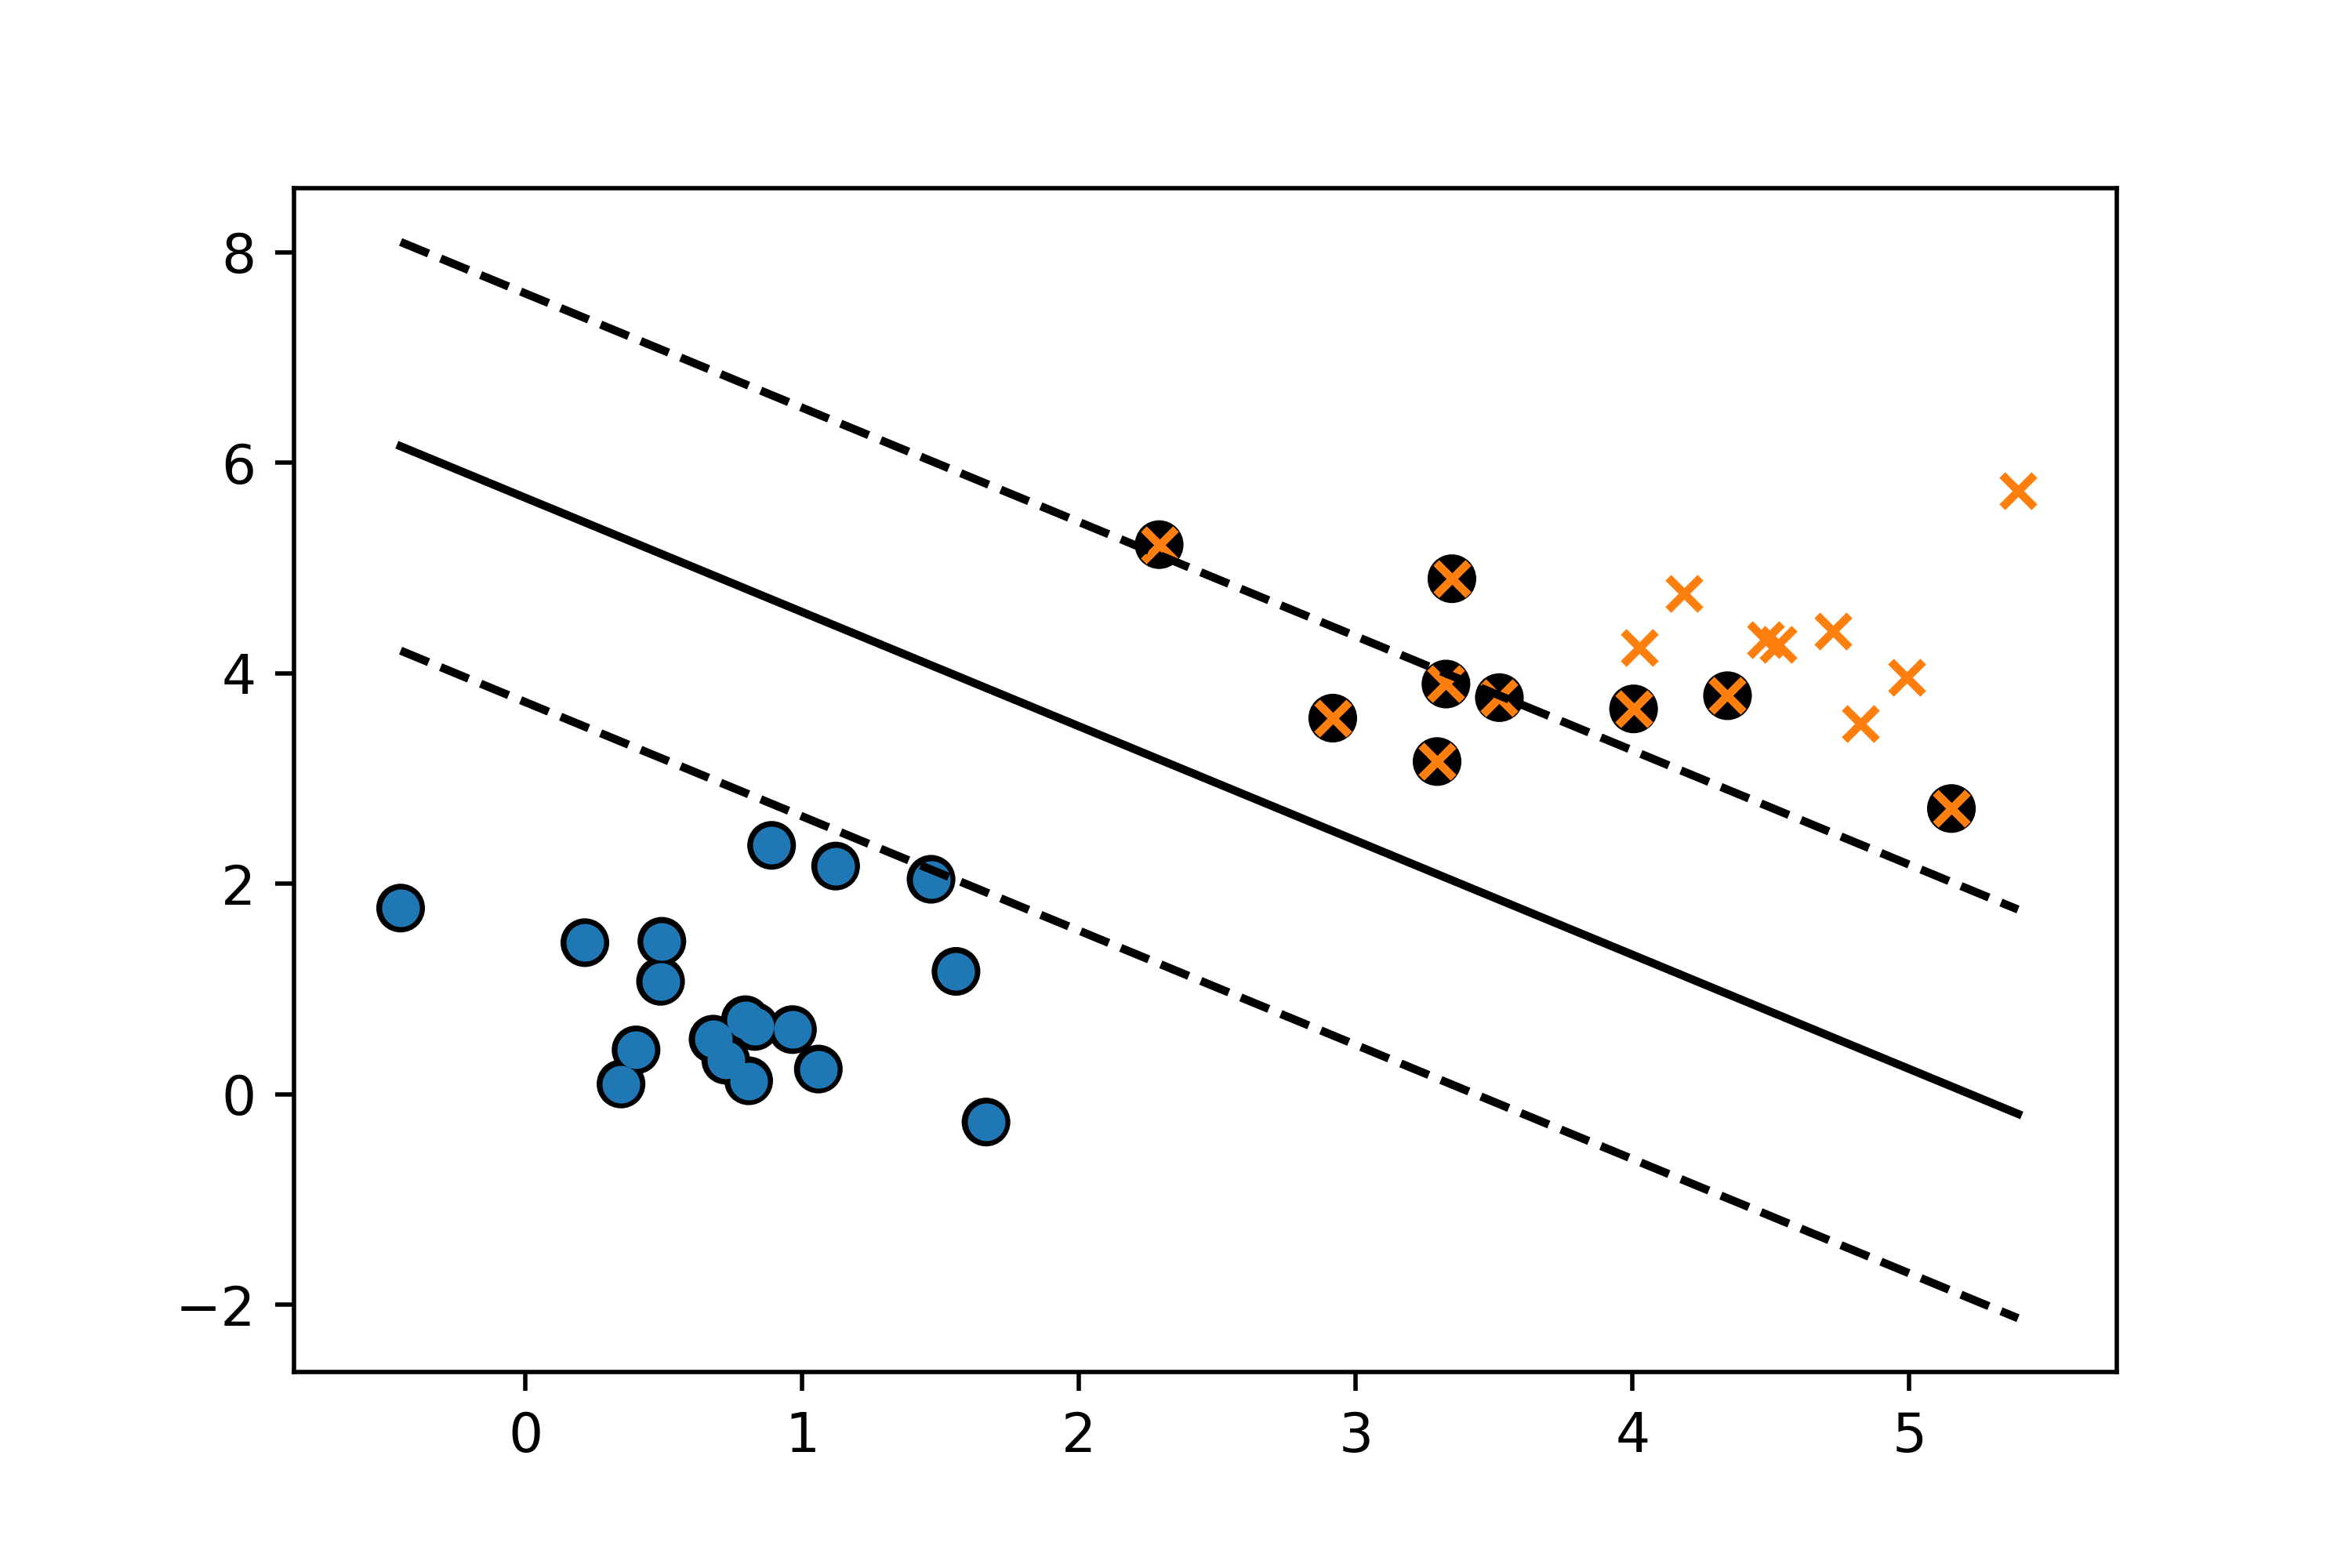
\includegraphics[scale=0.5]{SVM}
	\caption{مسئله حاشیه سخت در ماشین بردار پشتیبان}
	\label{fig:SVM}
\end{figure}



% Chapter 3 KNN-LSTSVM

\chapter{روش پیشنهادی}\label{ch:3}
\section{مقدمه}\label{sec:3:1}
روش پیشنهادی در این فصل ارائه می‌شود.
\section{تیتر 1}\label{sec:3:2}
یک زیربخش در سطح ۱
\subsection{تیتر 2}\label{sec:3:2:1}
یک زیربخش در سطح ۲
\subsubsection{تیتر 3}\label{sec:3:2:1:1}
یک ریزبخش در سطح ۳

% This chapter presents the proposed method.

\chapter{نتایج}\label{ch:4}
\section{معرفی مجموعه داده‌ها}\label{sec:4:1}
جدول \ref{tab:1} مشخصات مجموعه داده‌ها برای ارزیابی روش پیشنهادی را نشان می‌دهد. 

\begin{table}[!h]
	\centering
	\caption{مشخصات مجموعه داده‌ها برای ارزیابی روش}
	%\tabcolsep=0.11cm
	\begin{tabular}{l c c c c}
		\hline
		% after \\: \hline or \cline{col1-col2} \cline{col3-col4} ...
		مجموعه داده & تعداد نمونه‌ها & نمونه‌های مثبت & نمونه‌های منفی &تعداد ویژگی‌ها \\
		\hline
	\lr{{Austrailian}} & {690} & {307} & {383} & {14} \\
	\lr{{Heart-Statlog}} & {270} & {120} & {150} & {13} \\
	\lr{{Hepatits}} & {155} & {32} & {123} & {19} \\
	\lr{{Pima-Indian}} & {768} & {268} & {500} & {8} \\
	\lr{{Titanic}} & {891} & {342} & {549} & {7} \\
	\lr{{Votes}} & {435} & {267} & {168} & {16} \\
	\lr{{Wdbc}} & {569} & {212} & {357} & {30} \\
		\hline
	\end{tabular}
	
	\label{tab:1}
\end{table}


% Conclusion and future work

\chapter{نتیجه‌گیری}\label{ch:5}

\section{مقدمه}\label{sec:5:1}



% References
% References

% Add references to TOC
\addcontentsline{toc}{chapter}{مراجع}

\bibliographystyle{ieeetr-fa}
\bibliography{references/ref_bibtex}


% Glossaries
\printglossary
\printabbreviation

% Change lines space after glossary
\baselineskip=0.9cm

% English abstract
% English Abstract
\pagestyle{plain}

\addcontentsline{toc}{chapter}{چکیده انگلیسی}

\begin{latin}
	
\section*{Abstract}
Write an English abstract of your thesis here.
	
\vspace{2cm}
\noindent \textbf{Keywords:}
TeX template, Artificial Intelligence
	
\end{latin}

% English title page
% English title page

\thispagestyle{empty}

\begin{center}
	
	\begin{latin}
		
		{\LARGE \bf ISLAMIC AZAD UNIVERSITY}
		\\[1cm]
		{\Large North Tehran Branch}
		\\[1cm]
		{\Large "M.Sc" Thesis}
		\\[2cm]
		
		{\Large Research Title}
		\\[.5cm]
		{.....................................}
		\\[1cm]
		{\Large Supervisor}
		\\[.5cm]
		{...............}
		\\[1cm]
		{\Large Consulting Supervisor}
		\\[.5cm]
		{...............}
		\\[1cm]
		{\Large By}
		\\[.5cm]
		{...............}
		\\[1cm]
		Autumn 2018
		
	\end{latin}
\end{center}


\end{document}